This chapter presents the corification of a modeling language for the requirements phase using the CORE metamodel. We describe the steps taken to corify UCM in Section~\ref{sec:3.1}. We also present the weaving algorithm specific for UCM in the context of CORE in Section~\ref{sec:3.2}.

\section{Corification of UCM} \label{sec:3.1}

Abstract and concrete classes of the CORE metamodel are utilized differently when corifying a modeling language. The abstract classes \textit{\cls COREModel}, \textit{\cls COREModelElement}, and \textit{\cls COREPattern} serve as extension points and are intended to be subclassed by a modeling language. This enables the addition of arbitrary modeling languages to CORE and also uniform treatment of pattern-based composition. The remaining abstract classes \textit{\cls COREModelComposition}, \textit{\cls COREModelElementComposition}, and \textit{\cls CORELink} are used within the CORE metamodel and seldom subclassed by a modeling language. On the contrary, concrete classes are designed to be used exactly as it is in the corified modeling languages. They provide the necessary mechanisms for model extensions and reuses, feature and impact modeling, as well as a way to implements and visualizes these concepts in its modeling tool.

\begin{figure}
	\centering
	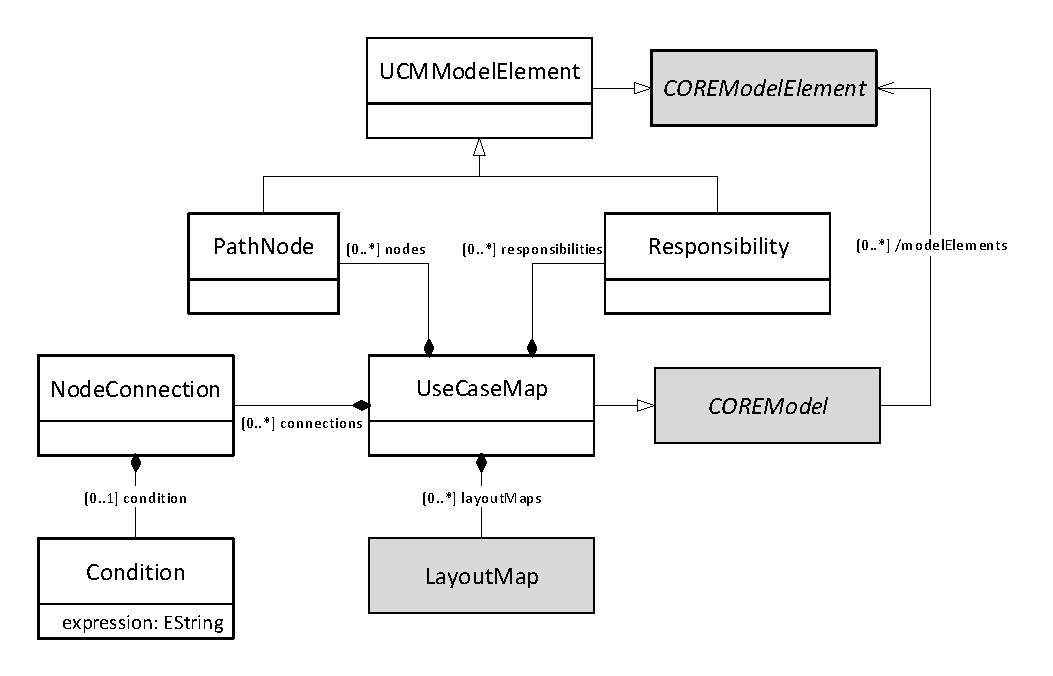
\includegraphics[scale=0.5]{fig_3_1.pdf}
	\caption{Extension of the CORE metamodel by UCM}
	\label{fig:3.1}
\end{figure}

We follow the URN specification~\cite{itu2012151} closely in corifying the UCM metamodel. Figure~\ref{fig:3.1} shows a partial view of the corified UCM metamodel, focusing on the elements that extend the CORE metamodel through subclassing (from an existing metaclass in the modeling language to an abstract CORE metaclass \footnote{The gray elements in the figures are the classes that derived from the CORE metamodel.}). By subclassing the necessary abstract classes of the CORE metamodel, UCM is able to provide all the properties of CORE:

\begin{itemize}
	\setlength{\parskip}{0pt} \setlength{\itemsep}{0pt}
	\item A UCM model may now belong to a concern by realizing at least one of its features.
	\item A realization model could potentially have impacts on high-level goals.
	\item A UCM model may extend another UCM model that belongs to a different feature.
	\item A UCM model may reuse another UCM model that belongs to a different concern.
\end{itemize}

Reusing a concern from a UCM model prompts the feature selection process, by asking the feature that the UCM model realizes to reuse the other concern with the selection of feature(s) it wants to reuse. The reusing UCM model then establishes the mappings to the reused UCM model that realizes the reused features. This is achieved as follows. The root element {\cls UseCaseMap} subclasses \textit{\cls COREModel}, which makes it part of a {\cls COREConcern} (see Figure~\ref{fig:2.1}, association between {\cls COREConcern} and {\cls COREModel}). This allows a UCM to realize a feature (see Figure~\ref{fig:2.2}, {\cls COREModel} realizes {\cls COREFeature}) within a concern. Therefore, the concern can create a {\cls COREReuse} to reuse another concern. The reusing UCM then creates a {\cls COREModelReuse} that has a direct association to the created {\cls COREReuse} and a \textit{\cls COREConfiguration} that selects the desired features from the reused concern. The CORE modeling tool then composes the UCM models of the reused concern that realize the selected features to generate a single woven user-tailored UCM model of the reused concern. Mappings to the model elements of this generated model are established using the class {\cls COREMapping}, consequently allowing the reusing UCM to customize the generated UCM model of the reused concern.

\begin{figure}
	\centering
	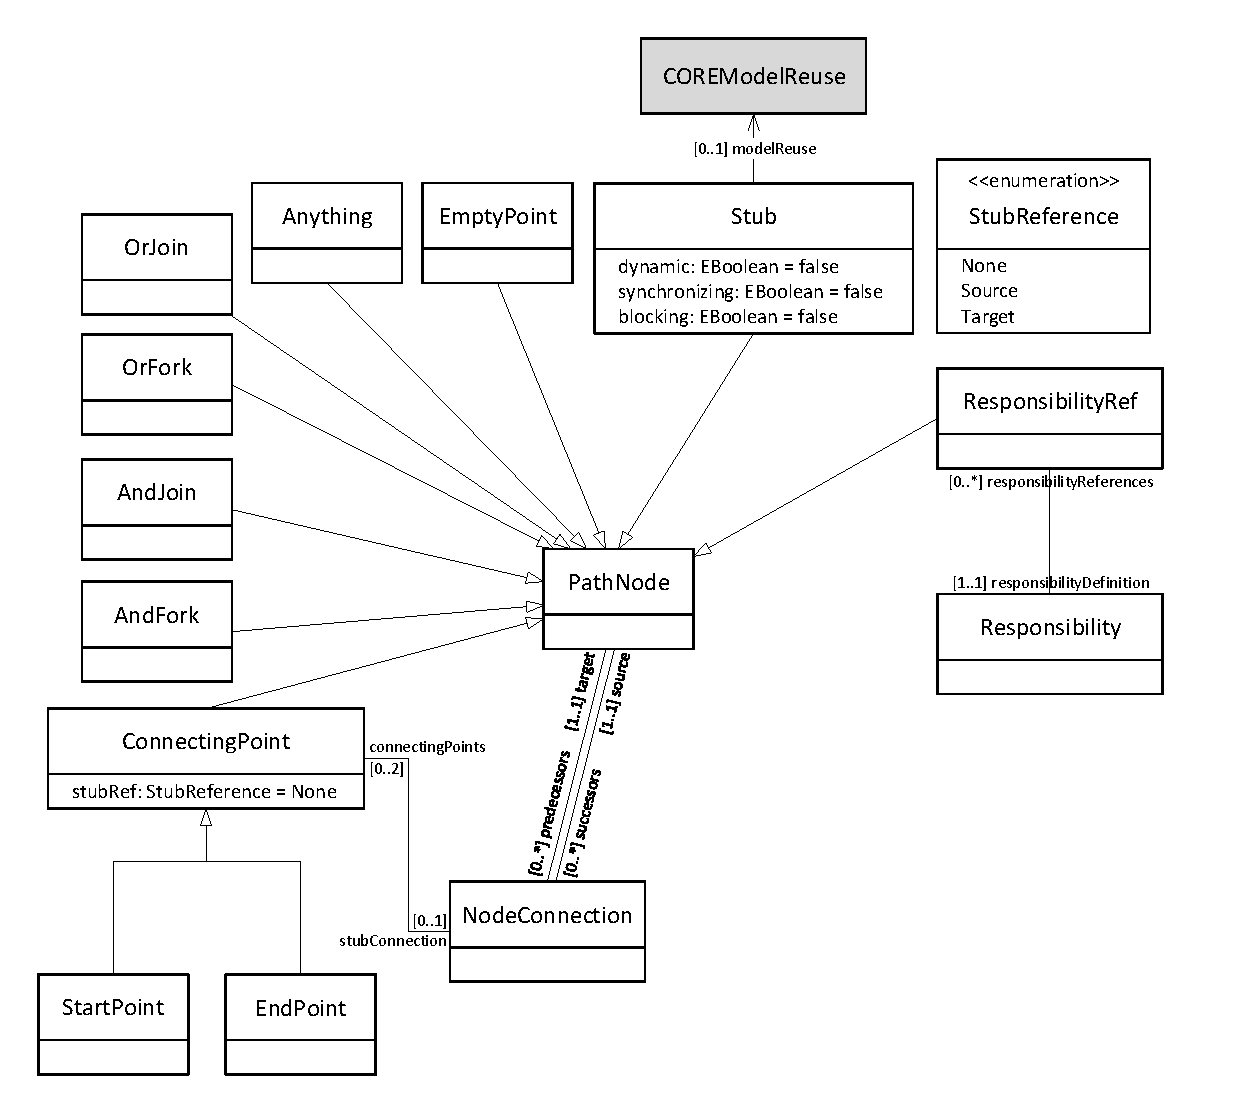
\includegraphics[scale=0.5]{fig_3_2.pdf}
	\caption{Path nodes for corified UCM}
	\label{fig:3.2}
\end{figure}

A standard UCM consists of {\cls PathNode}, {\cls Responsibility}, and {\cls NodeConnection}. {\cls LayoutMap} is added as part of the composition to allow positioning of the elements for viewing. We omit the inclusion of certain elements such as {\cls Component}, {\cls Timer}, and {\cls FailurePoint} to limit the scope of this thesis. On the contrary, {\cls PluginBinding} is excluded on purpose since we utilize {\cls COREMapping} as our approach to bind separate UCMs to {\cls Stub}. We incorporate several changes to the path nodes to support aspect-oriented modeling and reuse. Figure~\ref{fig:3.2} illustrates the addition of {\cls Anything} and {\cls ConnectingPoint}, as well as a directed association from {\cls Stub} to {\cls COREModelReuse}, to the UCM metamodel.

\textbf{\cls Anything:} We included the {\cls Anything} pointcut element from the extended AoUCM metamodel~\cite{mussbacher2011aspect}. {\cls Anything} acts as a wild card and can represent a subset of nodes in a path. This is useful for facilitating complex model weaving, as it allows any sequence of UCM model elements, including an empty sequence, to be matched.

\textbf{\cls ConnectingPoint:} We established a new path element to the metamodel. {\cls ConnectingPoint} is used to replace {\cls PluginBinding} and serves as an intermediate node that represents either a {\cls StartPoint} or an {\cls EndPoint}. By default, an actual start or end point within a UCM does not have a reference to a stub, hence the default value for {\cls StubReference} is {\cls None}. Instead, when we have a {\cls NodeConnection} that connects an element with a stub, then a hidden connecting point is automatically attached to the node connection (and deleted upon removal of the connection). Each node connection can have at most two connecting points if both the source and target nodes of the connection are stubs. Incoming connection to a stub generates a hidden end point with the value of {\cls stubRef} set to {\cls Target}, whereas outgoing connection from a stub generates a hidden start point with the value of {\cls stubRef} set to {\cls Source}. These hidden points allow us to define composition specifications through customization mappings.

\begin{figure}
	\centering
	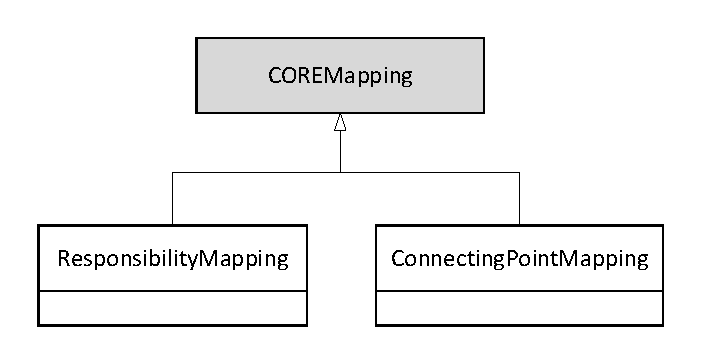
\includegraphics[scale=0.5]{fig_3_3.pdf}
	\caption{Customization mappings for corified UCM}
	\label{fig:3.3}
\end{figure}

Since we are using {\cls COREMapping} to specify customizations, it is necessary for {\cls UCMModelElement} to subclass \emph{\cls COREModelElement}. That way, all subclasses of {\cls UCMModelElement} (i.e., {\cls PathNode} and {\cls Responsibility}) can be used as source and destination classes for {\cls COREMapping}. As shown in Figure~\ref{fig:3.3}, we defined the composition specifications for specific UCM model elements: {\cls Responsibility} and {\cls ConnectingPoint}. They were selected so that we can compose UCM models based on the mappings of these elements. This leads us to the next section where we describe in detail how model composition is achieved through weaving.

\section{UCM Weaving} \label{sec:3.2}

As explained in Section~\ref{sec:2.1}, the role of the weaver is to facilitate model extensions and reuses. We offer two options when mapping elements between UCMs: (i) direct mapping of responsibilities; and (ii) cross mapping of connecting points. Cross mapping is necessary because of the nature of start and end points, where a start point of a UCM maps to an end point of a stub, and vice versa. A stub can be perceived as being superimposed with an end point followed by a start point, and those points collapsed into a point that is the stub \cite{buhr1995use}. Here, the hidden end point of a stub represents the incoming connection and it signifies the end of the sequence before the stub, and the hidden start point of a stub represents the outgoing connection and it signifies the start of the sequence after the stub. Both options have different procedures when weaving.

\subsection{Weaving Algorithm}

The algorithms presented here are specific for single weaving, meaning that a composition is performed from one model (\emph{UCM}\textsubscript{1}) to another model (\emph{UCM}\textsubscript{2}). This action can be chained together with other compositions, even with the hierarchical structure of the concern features. Here, we specify the subscript \textsubscript{1} for the model elements of a UCM the weaver composes from, and the subscript \textsubscript{2} for the model elements of a UCM the weaver composes to. \emph{UCM}\textsubscript{1} and \emph{UCM}\textsubscript{2} are merged prior to weaving, retaining all the path nodes and node connections from both models. Then the weaver iterates through the available composition specifications and executes the algorithms based on the specific type of mapping. The output of the woven model results in the amalgamation of UCMs based on the composition specification defined by the designer of the models, as well as the selected features of the concern by the user.

\subsubsection{Responsibility Mapping} \label{sec:3.2.1.1}

\begin{algorithm}
    \caption{Weaving Algorithm: Responsibility Mapping}
    \label{alg:1}
	\begin{algorithmic}[1]
	    \Function{WeaveResponsibilityMapping}{\emph{ucm}, \emph{composition}}
			\State \emph{node}\textsubscript{1} $\gets$ get first node of \emph{composition} mapping (\emph{from})
			\State \emph{node}\textsubscript{2} $\gets$ get second node of \emph{composition} mapping (\emph{to})
			\State mark \emph{node}\textsubscript{2} as visited
			\State indicate start point has not been encountered
			\State indicate end point has not been encountered
			\State call \Call{TraverseToSource}{\emph{ucm}, \emph{node}\textsubscript{2}, \emph{node}\textsubscript{1}}
			\State call \Call{TraverseToTarget}{\emph{ucm}, \emph{node}\textsubscript{2}, \emph{node}\textsubscript{1}}
			\State remove \emph{node}\textsubscript{1} from \emph{ucm}
		\EndFunction
		
		\Function{TraverseToSource}{\emph{ucm}, \emph{node}\textsubscript{2}, \emph{node}\textsubscript{1}}
			\For{each predecessor of \emph{node}\textsubscript{2}}
				\State \emph{sourceNode} $\gets$ get source node of predecessor
				\If{linkage exists from previous mapping} \label{alg:1.1}
					\State set the source of \emph{node}\textsubscript{2}'s connection to \emph{node}\textsubscript{1}'s predecessor
					\State disable linkage
					\State skip this loop
				\EndIf \label{alg:1.2}
				\If{\emph{sourceNode} is visited} \label{alg:1.3}
					\State skip this loop
				\ElsIf{\emph{sourceNode} is not {\cls Anything}}
					\State mark \emph{sourceNode} as visited
				\EndIf \label{alg:1.4}
				\If{\emph{sourceNode} is {\cls StartPoint} and start point is not encountered} \label{alg:1.5}
					\If{visibility of \emph{sourceNode} is {\cls Concern}}
						\State set the source of \emph{node}\textsubscript{2}'s connection to \emph{node}\textsubscript{1}'s predecessor
						\State remove \emph{sourceNode} from \emph{ucm}
						\State indicate start point has been encountered
					\EndIf \label{alg:1.6}
				\ElsIf{\emph{sourceNode} is {\cls Anything}} \label{alg:1.7}
					\State set the source of \emph{node}\textsubscript{2}'s connection to \emph{node}\textsubscript{1}'s predecessor
					\If{\emph{sourceNode} does not have any predecessor}
						\State remove \emph{sourceNode} from \emph{ucm}
					\EndIf \label{alg:1.8}
				\Else
					\State recursively call \Call{TraverseToSource}{\emph{ucm}, \emph{sourceNode}, \emph{node}\textsubscript{1}} \label{alg:1.9}
				\EndIf
			\EndFor
		\EndFunction
		
		\algstore{alg1}
	\end{algorithmic}
\end{algorithm}

\begin{algorithm}                     
	\begin{algorithmic}[1]
		\algrestore{alg1}
		
		\Function{TraverseToTarget}{\emph{ucm}, \emph{node}\textsubscript{2}, \emph{node}\textsubscript{1}}
			\For{each successor of \emph{node}\textsubscript{2}}
				\State \emph{targetNode} $\gets$ get target node of successor
				\If{\emph{targetNode} is visited} \label{alg:1.10}
					\State skip this loop
				\ElsIf{\emph{targetNode} is not {\cls Anything}}
					\State mark \emph{targetNode} as visited
				\EndIf \label{alg:1.11}
				\If{\emph{targetNode} is {\cls Endpoint} and end point is not encountered} \label{alg:1.12}
					\If{visibility of \emph{targetNode} is {\cls Concern}}
						\State set the target of \emph{node}\textsubscript{2}'s connection to \emph{node}\textsubscript{1}'s successor
						\State remove \emph{targetNode} from \emph{ucm}
						\State indicate end point has been encountered
					\EndIf \label{alg:1.13}
				\ElsIf{\emph{targetNode} is {\cls Anything}} \label{alg:1.14}
					\State set the target of \emph{node}\textsubscript{2}'s connection to \emph{node}\textsubscript{1}'s successor
					\If{\emph{targetNode} does not have any successor}
						\State remove \emph{targetNode} from \emph{ucm}
					\EndIf \label{alg:1.15}
				\ElsIf{\emph{targetNode} exists in \emph{composition} mapping (\emph{to})} \label{alg:1.16}
					\State copy node connection of successor
					\State set the target of copied connection to \emph{node}\textsubscript{1}'s successor
					\State add the copied connection to \emph{ucm}
					\State enable linkage to next mapping \label{alg:1.17}
				\Else
					\State recursively call \Call{TraverseToTarget}{\emph{ucm}, \emph{targetNode}, \emph{node}\textsubscript{1}} \label{alg:1.18}
				\EndIf
			\EndFor
		\EndFunction
	\end{algorithmic}
\end{algorithm}

Mapping with responsibilities allows for model extensions between parent and child UCMs. Composition specification can be defined by mapping from a parent UCM's responsibility to a child UCM's responsibility. Algorithm~\ref{alg:1} illustrates the procedure of weaving for responsibility mappings. The function \emph{WeaveResponsibilityMapping} initiates the process by identifying the mapped responsibilities (\emph{from} \emph{UCM}\textsubscript{1} \emph{to} \emph{UCM}\textsubscript{2}), and traversal begins from the point of \emph{responsibility}\textsubscript{2} in both directions: (i) toward predecessors until start point encountered; and (ii) toward successors until end point encountered. A UCM is represented as a directed graph, with possible cycles via {\cls OrFork}s and {\cls OrJoin}s. As such, we implemented a depth-first search approach for traversing the graph through recursion (lines~\ref{alg:1.9} and~\ref{alg:1.18}), and a mechanism to determine whether a node has been explored (lines~\ref{alg:1.3}-\ref{alg:1.4} and~\ref{alg:1.10}-\ref{alg:1.11}).

Furthermore, we allow multiple consecutive mappings between two UCM models. The path of a UCM may consist of mapped responsibilities interspersed with other path nodes. While traversing forward, lines~\ref{alg:1.16}-\ref{alg:1.17} handle the next mapped responsibility. If exist, forward traversal stops for this specific composition and appropriate nodes are connected between \emph{UCM}\textsubscript{1} and \emph{UCM}\textsubscript{2}. For subsequent mappings, lines~\ref{alg:1.1}-\ref{alg:1.2} handle the linkage from previous mappings, and backward traversal stops at the point of mapped responsibilities and appropriate nodes are connected between \emph{UCM}\textsubscript{1} and \emph{UCM}\textsubscript{2}. This pattern continues until the weaver reaches end point, whereby the predecessor of \emph{UCM}\textsubscript{2}'s end point connects to the successor of mapped responsibility (\emph{from}) \emph{UCM}\textsubscript{1} and this end point gets deleted (lines~\ref{alg:1.12}-\ref{alg:1.13}). Same goes for backward traversal until the weaver reaches start point (lines~\ref{alg:1.5}-\ref{alg:1.6}). Lastly, mapped responsibility (\emph{to}) \emph{UCM}\textsubscript{2} retains while mapped responsibility (\emph{from}) \emph{UCM}\textsubscript{1} gets deleted for the final woven UCM model.

UCM may have multiple start points merging to a path, or a path may branch to multiple end points. In this case, we allow a start or end point to set its visibility level. By default, connecting point is given the visibility of {\cls Concern} that signifies the start or end point is only visible when viewing a UCM model for a specific feature of a concern, but disappears after the composition process. The other option is {\cls Public} for global visibility and is used to retain the start or end point even after the composition process---the weaver would just ignore {\cls Public} connecting points and proceed to other branches. This feature is useful in defining multiple entry points, or alternative exit strategies, for a scenario.

Complex scenario model composition is also possible with the help of {\cls Anything}. An anything node can represent a subset of nodes in a path and is commonly used in \emph{UCM}\textsubscript{2} to capture the actual nodes that are specified in \emph{UCM}\textsubscript{1}. If an anything node is encountered during traversal, lines~\ref{alg:1.7}-\ref{alg:1.8} and~\ref{alg:1.14}-\ref{alg:1.15} signals the end of exploration and treat it as an end point. The difference is that the algorithm checks whether the anything node is still connected to other nodes before removal. This is necessary because an anything node has a predecessor node and a successor node, and typically surrounded by forks and joins (loop cycle). Both sides have to be traversed and dealt with before removing the anything node from the woven model.

\subsubsection{Connecting Point Mapping}

\begin{algorithm}
	\caption{Weaving Algorithm: Connecting Point Mapping}
	\label{alg:2}
	\begin{algorithmic}[1]
		\Function{WeaveConnectingPointMapping}{\emph{ucm}, \emph{composition}}
			\State \emph{node}\textsubscript{1} $\gets$ get first node of \emph{composition} mapping (\emph{from})
			\State \emph{node}\textsubscript{2} $\gets$ get second node of \emph{composition} mapping (\emph{to})
			\If{\emph{node}\textsubscript{1} is {\cls StartPoint}}
				\If{\emph{node}\textsubscript{1} is connected to a stub} \label{alg:2.1}
					\State call \Call{ExtendingStub\_End}{\emph{ucm}, \emph{node}\textsubscript{2}, \emph{node}\textsubscript{1}} \label{alg:2.2}
				\ElsIf{\emph{node}\textsubscript{2} is connected to a stub} \label{alg:2.3}
					\State call \Call{ReusingStub\_Start}{\emph{ucm}, \emph{node}\textsubscript{2}, \emph{node}\textsubscript{1}} \label{alg:2.4}
				\EndIf
			\ElsIf{\emph{node}\textsubscript{1} is {\cls EndPoint}}
				\If{\emph{node}\textsubscript{1} is connected to a stub} \label{alg:2.5}
					\State call \Call{ExtendingStub\_Start}{\emph{ucm}, \emph{node}\textsubscript{2}, \emph{node}\textsubscript{1}} \label{alg:2.6}
				\ElsIf{\emph{node}\textsubscript{2} is connected to a stub} \label{alg:2.7}
					\State call \Call{ReusingStub\_End}{\emph{ucm}, \emph{node}\textsubscript{2}, \emph{node}\textsubscript{1}} \label{alg:2.8}
				\EndIf
			\EndIf
		\EndFunction
		
		\Function{ExtendingStub\_End}{\emph{ucm}, \emph{node}\textsubscript{2}, \emph{node}\textsubscript{1}} \label{alg:2.9}
			\State \emph{source}\textsubscript{2} $\gets$ get source node of \emph{node}\textsubscript{2}
			\State \emph{source}\textsubscript{1} $\gets$ get source node of \emph{node}\textsubscript{1} via stub connection
			\State \emph{target}\textsubscript{1} $\gets$ get target node of \emph{node}\textsubscript{1} via stub connection
			\State call \Call{MergePaths}{\emph{source}\textsubscript{2}, \emph{source}\textsubscript{1}, \emph{target}\textsubscript{1}, \emph{node}\textsubscript{1}, \emph{node}\textsubscript{1}}
			\State remove \emph{node}\textsubscript{2} from \emph{ucm}
		\EndFunction \label{alg:2.10}
		
		\Function{ReusingStub\_Start}{\emph{ucm}, \emph{node}\textsubscript{2}, \emph{node}\textsubscript{1}} \label{alg:2.11}
			\State \emph{target}\textsubscript{1} $\gets$ get target node of \emph{node}\textsubscript{1}
			\State \emph{target}\textsubscript{2} $\gets$ get target node of \emph{node}\textsubscript{2} via stub connection
			\State \emph{source}\textsubscript{2} $\gets$ get source node of \emph{node}\textsubscript{2} via stub connection
			\State call \Call{SplitPaths}{\emph{target}\textsubscript{1}, \emph{target}\textsubscript{2}, \emph{source}\textsubscript{2}, \emph{node}\textsubscript{2}, \emph{node}\textsubscript{1}}
			\State remove \emph{node}\textsubscript{1} from \emph{ucm}
		\EndFunction \label{alg:2.12}
		
		\Function{ExtendingStub\_Start}{\emph{ucm} \emph{node}\textsubscript{2}, \emph{node}\textsubscript{1}} \label{alg:2.13}
			\State \emph{target}\textsubscript{2} $\gets$ get target node of \emph{node}\textsubscript{2}
			\State \emph{target}\textsubscript{1} $\gets$ get target node of \emph{node}\textsubscript{1} via stub connection
			\State \emph{source}\textsubscript{1} $\gets$ get source node of \emph{node}\textsubscript{1} via stub connection
			\State call \Call{SplitPaths}{\emph{target}\textsubscript{2}, \emph{target}\textsubscript{1}, \emph{source}\textsubscript{1}, \emph{node}\textsubscript{1}, \emph{node}\textsubscript{1}}
			\State remove \emph{node}\textsubscript{2} from \emph{ucm}
		\EndFunction \label{alg:2.14}
		
		\algstore{alg2}
	\end{algorithmic}
\end{algorithm}

\begin{algorithm}                     
	\begin{algorithmic}[1]
		\algrestore{alg2}
		
		\Function{ReusingStub\_End}{\emph{ucm}, \emph{node}\textsubscript{2}, \emph{node}\textsubscript{1}} \label{alg:2.15}
			\State \emph{source}\textsubscript{1} $\gets$ get source node of \emph{node}\textsubscript{1}
			\State \emph{source}\textsubscript{2} $\gets$ get source node of \emph{node}\textsubscript{2} via stub connection
			\State \emph{target}\textsubscript{2} $\gets$ get target node of \emph{node}\textsubscript{2} via stub connection
			\State call \Call{MergePaths}{\emph{source}\textsubscript{1}, \emph{source}\textsubscript{2}, \emph{target}\textsubscript{2}, \emph{node}\textsubscript{2}, \emph{node}\textsubscript{1}}
			\State remove \emph{node}\textsubscript{1} from \emph{ucm}
		\EndFunction \label{alg:2.16}
		
		\Function{SplitPaths}{\emph{target}, \emph{target}$'$, \emph{source}$'$, \emph{node}, \emph{node}$'$}
			\If{\emph{target}$'$ is {\cls Stub}} \label{alg:2.17}
				\State mark \emph{target}$'$ as removable stub
				\State set target node of \emph{node}'s stub connection to \emph{target} \label{alg:2.18}
			\ElsIf{\emph{target}$'$ is {\cls AndFork} or {\cls OrFork}} \label{alg:2.19}
				\State create node connection between \emph{target}$'$ and \emph{target} \label{alg:2.20}
			\Else \label{alg:2.21}
				\State \emph{referenceStub} $\gets$ get target node of \emph{node}$'$ via stub connection
				\State \emph{forkNode} $\gets$ \textbf{if} \emph{referenceStub} is dynamic \textbf{then} create {\cls AndFork} \textbf{else} {\cls OrFork}
				\State place \emph{forkNode} in between \emph{source}$'$ and \emph{target}$'$
				\State create node connection between \emph{forkNode} and \emph{target}$'$
				\State create node connection between \emph{forkNode} and \emph{target}
				\State set target node of \emph{node}'s stub connection to \emph{forkNode}
			\EndIf \label{alg:2.22}
		\EndFunction
		
		\Function{MergePaths}{\emph{source}, \emph{source}$'$, \emph{target}$'$, \emph{node}, \emph{node}$'$}
			\If{\emph{source}$'$ is {\cls Stub}} \label{alg:2.23}
				\State mark \emph{source}$'$ as removable stub
				\State set source node of \emph{node}'s stub connection to \emph{source} \label{alg:2.24}
			\ElsIf{\emph{source}$'$ is {\cls AndJoin} or {\cls OrJoin}} \label{alg:2.25}
				\State create node connection between \emph{source} and \emph{source}$'$ \label{alg:2.26}
			\Else \label{alg:2.27}
				\State \emph{referenceStub} $\gets$ get source node of \emph{node}$'$ via stub connection
				\State \emph{joinNode} $\gets$ \textbf{if} \emph{referenceStub} is synchronizing \textbf{then} create {\cls AndJoin} \textbf{else} {\cls OrJoin}
				\State place \emph{joinNode} in between \emph{source}$'$ and \emph{target}$'$
				\State create node connection between \emph{source}$'$ and \emph{joinNode}
				\State create node connection between \emph{source} and \emph{joinNode}
				\State set source node of \emph{node}'s stub connection to \emph{joinNode}
			\EndIf \label{alg:2.28}
		\EndFunction
	\end{algorithmic}
\end{algorithm}

Mapping with connecting points allows for model extensions between parent and child UCMs and also model reuses from UCMs of other concerns. Algorithm~\ref{alg:2} illustrates the procedure of weaving for connecting point mappings. The function \emph{WeaveConnectingPointMapping} initiates the process by identifying the mapped connecting points (\emph{from} \emph{UCM}\textsubscript{1} \emph{to} \emph{UCM}\textsubscript{2}), and determine the type of composition to be performed based on whether the connecting points mapped from \emph{UCM}\textsubscript{1} are attached to a stub or not. If the mapped start and end points from \emph{UCM}\textsubscript{1} are attached to a stub (lines~\ref{alg:2.1}-\ref{alg:2.2} and~\ref{alg:2.5}-\ref{alg:2.6}), it means that the connecting points are hidden and belong to a stub in \emph{UCM}\textsubscript{1} and are mapped to actual end and start points of \emph{UCM}\textsubscript{2}, respectively (cross mapping). This type of composition is model extension. Vice versa for model reuse (lines~\ref{alg:2.3}-\ref{alg:2.4} and~\ref{alg:2.7}-\ref{alg:2.8}).

Model extension for stubs work differently compared with responsibilities. No traversal is required since there is no need to explore the whole graph, but the composition specification requires exactly two connecting point mappings for each stub to be complete---one for the start point and the second for end point. The weaver first obtain the pair of mappings for the stub. The initial mapping usually maps the end point of a stub \footnote{The end point of a stub symbolizes incoming node connection to the stub.} to the start point of a UCM, and the weaver executes lines~\ref{alg:2.9}-\ref{alg:2.10}. The second mapping usually maps the start point of a stub \footnote{The start point of a stub symbolizes outgoing node connection from the stub.} to the end point of a UCM, and the weaver executes lines~\ref{alg:2.13}-\ref{alg:2.14}.

Model reuse, on the other hand, operates in reversed orientation---obtaining the pairs of mappings that mapped the start and end points of \emph{UCM}\textsubscript{1} to the connecting points of a stub that is automatically generated in \emph{UCM}\textsubscript{2} when reusing \emph{UCM}\textsubscript{1}. To be precise, the automatically generated stub is always a static stub so that it can only hold a single UCM that originates from the reused concern. The weaver then executes lines~\ref{alg:2.11}-\ref{alg:2.12} and~\ref{alg:2.15}-\ref{alg:2.16}, respectively.

The execution procedure for both extension and reuse involves replacing a stub with plug-ins (sub-UCMs). Depending on the type of stub, it can bind either a single plug-in or multiple plug-ins. When facing a single plug-in bound to a stub, the weaver simply connects the nodes adjacent to the stub and nodes adjacent to the connecting points of a UCM, followed by the removal of the connecting points and the stub from the woven model (lines~\ref{alg:2.17}-\ref{alg:2.18} and~\ref{alg:2.23}-\ref{alg:2.24}). If there are two plug-ins bound to a stub, the weaver creates branches to link the two UCMs as parallel paths via fork and join nodes (lines~\ref{alg:2.21}-\ref{alg:2.22} and~\ref{alg:2.27}-\ref{alg:2.28}). The type of forks and joins being created is dependent on the type of stub. Synchronizing/blocking stubs produce branches that consist of {\cls AndFork} and {\cls AndJoin}, dynamic stubs produce branches that consist of {\cls AndFork} and {\cls OrJoin}, and static stubs produce branches that consist of {\cls OrFork} and {\cls OrJoin}. This process is also known as semantic flattening \cite{itu2012151}. Additional plug-ins bound to a stub are linked via the created forks and joins (lines~\ref{alg:2.19}-\ref{alg:2.20} and~\ref{alg:2.25}-\ref{alg:2.26}).
